\documentclass[conference]{IEEEtran}
% Add the compsoc option for Computer Society conferences.
%
% If IEEEtran.cls has not been installed into the LaTeX system files,
% manually specify the path to it like:
% \documentclass[conference]{../sty/IEEEtran}


% *** CITATION PACKAGES ***
%
\usepackage{cite}

% *** GRAPHICS RELATED PACKAGES ***
%
\usepackage[pdftex]{graphicx}
% declare the path(s) where your graphic files are
\graphicspath{{./images/}}
% and their extensions so you won't have to specify these with
% every instance of \includegraphics
\DeclareGraphicsExtensions{.png}

% *** MATH PACKAGES ***
%
\usepackage[cmex10]{amsmath}

% *** SPECIALIZED LIST PACKAGES ***
% *** SUBFIGURE PACKAGES ***
\usepackage[tight,footnotesize]{subfigure}

% *** PDF, URL AND HYPERLINK PACKAGES ***
%
\usepackage{url}

% *** TABLES ***
%



% correct bad hyphenation here
\hyphenation{op-tical net-works semi-conduc-tor}


\begin{document}
%
% paper title
% can use linebreaks \\ within to get better formatting as desired
\title{Lifelong Learning: A case study of punting balls}


% author names and affiliations
% use a multiple column layout for up to three different
% affiliations
\author{\IEEEauthorblockN{Ravikiran Janardhana}
\IEEEauthorblockA{Department of Computer Science\\
University of North Carolina at Chapel Hill\\
Email: ravikirn@cs.unc.edu}}

% conference papers do not typically use \thanks and this command
% is locked out in conference mode. If really needed, such as for
% the acknowledgment of grants, issue a \IEEEoverridecommandlockouts
% after \documentclass

% for over three affiliations, or if they all won't fit within the width
% of the page, use this alternative format:
% 

% make the title area
\maketitle

\begin{abstract}
%\boldmath
Designing robots that learn by themselves to perform complex real-world tasks is a still-open challenge for the field of Robotics and Artificial Intelligence. In this project, I use the case study of punting balls as a lifelong learning problem. The robot is fed with demonstrations of punting a variety of balls and records the target distanced acheived and updates the physics model of the punt with each demonstration. The learning process is continuous and not stagnant and as a result of this, the internal model needs to be bounded by a finite memory and we need to represent model/data in an efficient format. After the initial demonstrations, the robot is able to predict the launch velocity and the angle of elevation given any new ball and a target distance to reach. The efficient data representation of the model is achieved using the combination of Gaussian Mixture Models (GMM) and Gaussian Mixture Regression (GMR) and I show that the memory required to store the such an internal model compared to storing each of the individual demonstrations is substantially small. Using this physics model, the robot can predict the configuration to punt a new ball to reach a target distance with high accuracy.
\end{abstract}

\section{Introduction}
Throughout the last decades, the field of robotics has produced a large variety of approaches to automate and perform a variety of tasks. Despite significant progress in virtually all aspects of robotics science, most of today's robots are specialized to perform a narrow set of tasks in a very particular kind of environment. Most robots employ specialized controllers that have been carefully designed by hand, using extensive knowledge of the robot, its environment and its task. If one is interested in building autonomous multi-purpose robots, such approaches face some serious bottlenecks such as knowledge bottleneck (not aware of all the dynamics at design time), engineering bottleneck (most models are explictly hand coded) and tractability bottleneck (high computational complexity). 

Machine learning aims to overcome these limitations, by enabling a robot to collect its knowledge on-the-fly, through realworld experimentation. If a robot is placed in a novel, unknown environment, or faced with a novel tak for which no a priori solution is known, a robot that learns can collect new experiences, acquire new skills, and eventually perform new tasks all by itself. For example, in \cite{ref:1} a robot manipulator is described which learns to insert a peg in a hole without prior knowledge regarding the manipulator or the hole. Maes and Brooks \cite{ref:2} successfully applied learning techniques to coordinating leg motion for an insect-like robot. Their approach, too, operates in the absence of a model of the dynamics of the system. Learning techniques have frequently come to bear in situations where the physical world is extremely hard to model by hand (e.g., the characteristics of noisy sensors). For example, Pomerleau describes a computer system that learns to steer a vehicle driving at 55mph on public highways, based on input sensor data from a video camera \cite{ref:3}. Learning techniques have also successfully been applied to speed-up robot control, by observing the statistical regularities of "typical" situations (like typical robot and environment configurations), and compiling more compact controllers for the frequently encountered. For example, Mitchell \cite{ref:4} describes an approach in which a mobile robot becomes increasingly reactive, by using observations to compile fast rules out of a database of domain knowledge. 

However, there is a principle shortcoming in most of to date's rigorous learning approaches. Most of the robot control learning approaches focus on learning to achieve single, isolated performance tasks. If one is interested in learning with a minimum amount of initial knowledge, as is often the case in approaches to robot learning, such approaches have a critical limiting factor the number of training examples required for successful generalization. The more complex the task at hand and the lesser is known about the problem beforehand, the more training data is necessary to achieve the task. In many robotics domains the collection of training data is an expensive undertaking due to the slowness of robotics hardware. Hence, it does not surprise that the time required for real-world experimentation has frequently been found to be the limiting factor that prevents rigorous machine learning techniques from being truly successful in robotics. 

The task of learning from scratch can be significantly simplified by considering robots that face whole collections of control learning problems over their entire lifetime. In such a lifelong robot learning scenario \cite{ref:5, ref:6}, learning tasks are related in that they all play in the same environment, and that they involve the the same robot hardware. Lifelong learning scenarios open the opportunity for the transfer of knowledge across tasks. Complex tasks, which might require huge amounts of training data when faced in isolation, can conceivably be achieved much faster if a robot manages to exploit previously learned knowledge. For example, a lifelong learning robot might acquire general-purpose knowledge about itself and its environment, or acquire generally useful skills that can be applied in the context of multiple tasks. Such functions, once learned, can be applied to speed up learning in new tasks. 

In order to transfer knowledge across various tasks, first we need to have an efficient physical model representation of any task at hand rather than storing each of the individual demonstration as is. Also, it is expected that the robot continues to learn via new demonstrations and this places a limit on the amount of data it can store. In this project, I have used the example of punting a ball and analyzed the physical model required to replicate the punt trajectories. I present a novel method to store the punt physical model extracted using Gaussian Mixture Models (GMM) in an efficient matrix structure which can be later used to retrieve trajectories using Gaussian Mixture Regresstion given any new configuration. By doing so, I show that the memory required to store the model using my method is substantially smaller when compared to storing all of the trajectory data. I also show that the retrieved trajectory from this model is highly accurate without losing too much of information.

\section{Method}
\subsection{Physics model of a punt}
Equations for hang time and horizontal distance can be derived from the projectile equations of motion
\begin{equation}
y(t) = v_{y}t - \frac{1}{2}a_{y}t^{2}
\end{equation}
\begin{equation}
x(t) = v_{x}t
\end{equation}
where y and x are the height and horizontal displacements respectively, $v_{y}$ and $v_{x}$ are its vertical and horizontal velocities, $a_{y}$ is its vertical acceleration, and t is its time in flight. An expression for hang time, T, results from solving Eqn 1 for t when y = 0 and a = 9.8m/$s^{2}$ ,
\begin{equation}
T = \frac{2v_{0} sin(\theta_{0})}{9.8}
\end{equation}
where $v_{0}$ and $\theta_{0}$ are initial velocity and launch angle respectively. 

However, the above equations neglect air resistance which can lead to a substantial error when dealing in a practical environment. Air resistance, or drag, is a viscous force in a direction opposing the velocity of the projectile. Air drag, W, is given by the relation,
\begin{equation}
W = \frac{1}{2}\rho{C_{D}}Av^{2} 
\end{equation}
where $\rho$ is the air density, $C_{D}$ is the drag coefficient, A is the cross-sectional area of the projectile normal to the trajectory and v is the speed of the projectile relative to the air.

In order to include the drag into the physics model, the acceleration in x and y directions have to be suitably modified as below,
\begin{equation}
a_{x} = -C_{D}vv_{x}
\end{equation}
\begin{equation}
a_{y} = -C_{D}vv_{y} - g
\end{equation}
where g = 9.8m/$s^{2}$ and the negative sign indicates that these forces are acting against the launch velocity. 

% Table 1
\begin{table}[t]
\centering
\caption{Variation of Model parameters}
\begin{tabular}{  | c | c | c | c | c |}
  \hline
  Model & $v_{0}$ & $\theta_{0}$ & $max_{x}$ & $t_{total}$\\
  \hline 
  Without Drag  & 31.3 m/s  & 45$^{\circ}$ & 100.01 m & 4.52 secs  \\ 
  \hline
  With Drag  & 31.3 m/s  & 45$^{\circ}$ & 63.21 m & 3.6 secs  \\
  \hline
  With Drag Corrected  & 43.31 m/s  & 44$^{\circ}$ & 100.01 m & 4.7 secs  \\
  \hline
\end{tabular}
\label{tab:tab1}
\end{table}

%% Figure1
\begin{figure}[!t]
\centering
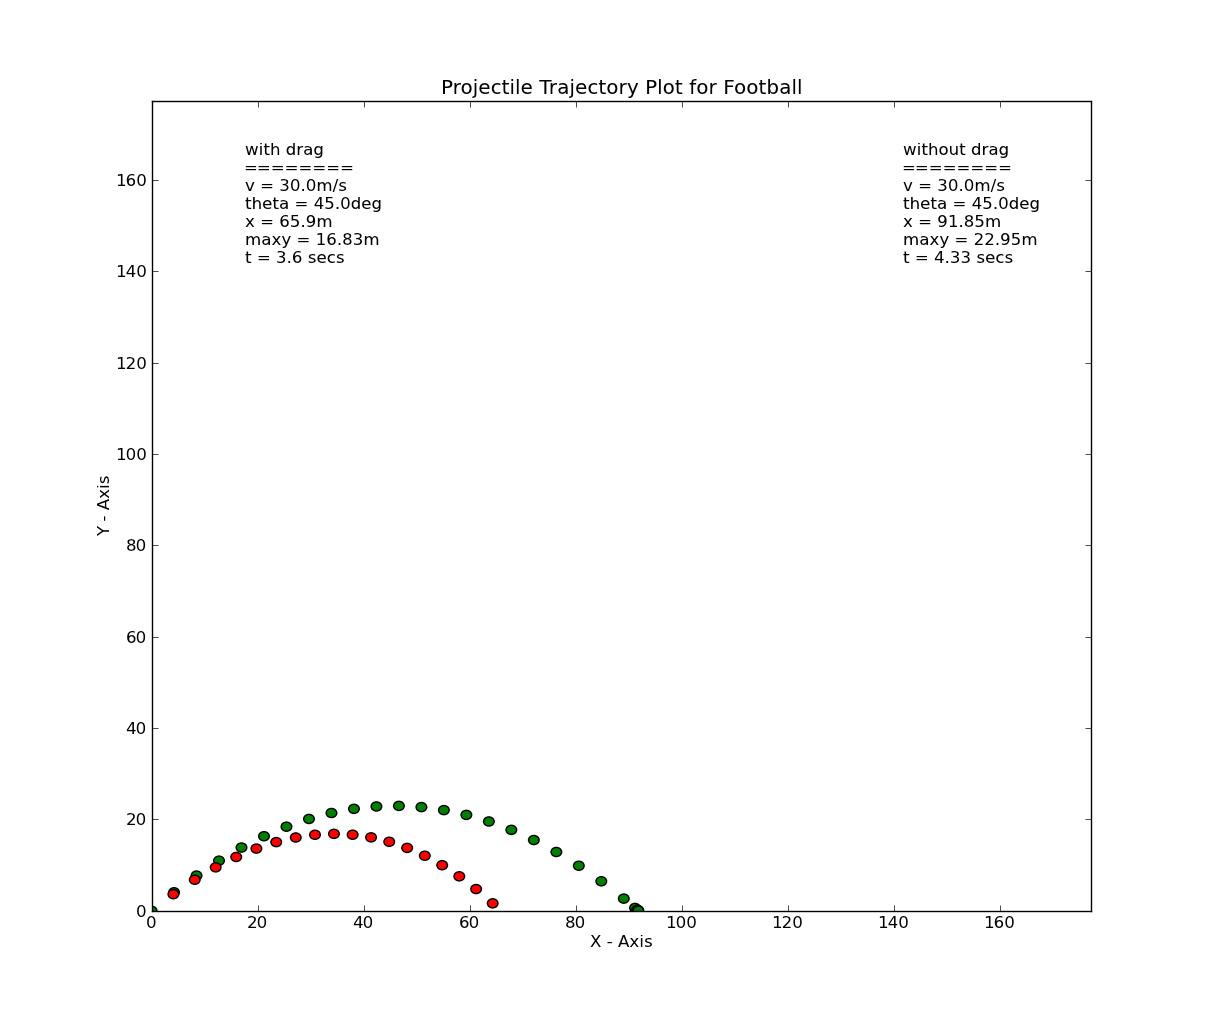
\includegraphics[width=3.5in]{fig1}
\caption{Projectile with and without drag}
\label{fig:fig1}
\end{figure}

Consider a scenario where the robot needs to predict the launch velocity and angle so that a football reaches a target distance of 100 meters assuming the Drag Coefficient $C_{D}$ in air is 0.006.  Table ~\ref{tab:tab1} shows the variation of maximum horizontal distance ($max_{x}$) and total time taken ($t_{total}$) by the projectile with and without taking drag forces into account. Using the learned model, the robot now predicts the correct launch velocity and angle to reach the target distance using a greedy optimizer. Figure ~\ref{fig:fig1} shows the pictorial representation of the scenario described by Table ~\ref{tab:tab1}.  



% An example of a double column floating figure using two subfigures.
% (The subfig.sty package must be loaded for this to work.)
% The subfigure \label commands are set within each subfloat command, the
% \label for the overall figure must come after \caption.
% \hfil must be used as a separator to get equal spacing.
% The subfigure.sty package works much the same way, except \subfigure is
% used instead of \subfloat.
%
%\begin{figure*}[!t]
%\centerline{\subfloat[Case I]\includegraphics[width=2.5in]{subfigcase1}%
%\label{fig_first_case}}
%\hfil
%\subfloat[Case II]{\includegraphics[width=2.5in]{subfigcase2}%
%\label{fig_second_case}}}
%\caption{Simulation results}
%\label{fig_sim}
%\end{figure*}
%
% Note that often IEEE papers with subfigures do not employ subfigure
% captions (using the optional argument to \subfloat), but instead will
% reference/describe all of them (a), (b), etc., within the main caption.


% An example of a floating table. Note that, for IEEE style tables, the 
% \caption command should come BEFORE the table. Table text will default to
% \footnotesize as IEEE normally uses this smaller font for tables.
% The \label must come after \caption as always.
%
%\begin{table}[!t]
%% increase table row spacing, adjust to taste
%\renewcommand{\arraystretch}{1.3}
% if using array.sty, it might be a good idea to tweak the value of
% \extrarowheight as needed to properly center the text within the cells
%\caption{An Example of a Table}
%\label{table_example}
%\centering
%% Some packages, such as MDW tools, offer better commands for making tables
%% than the plain LaTeX2e tabular which is used here.
%\begin{tabular}{|c||c|}
%\hline
%One & Two\\
%\hline
%Three & Four\\
%\hline
%\end{tabular}
%\end{table}


% Note that IEEE does not put floats in the very first column - or typically
% anywhere on the first page for that matter. Also, in-text middle ("here")
% positioning is not used. Most IEEE journals/conferences use top floats
% exclusively. Note that, LaTeX2e, unlike IEEE journals/conferences, places
% footnotes above bottom floats. This can be corrected via the \fnbelowfloat
% command of the stfloats package.



\section{Conclusion}
The conclusion goes here.




% conference papers do not normally have an appendix


% use section* for acknowledgement
\section*{Acknowledgment}


The authors would like to thank...





% trigger a \newpage just before the given reference
% number - used to balance the columns on the last page
% adjust value as needed - may need to be readjusted if
% the document is modified later
%\IEEEtriggeratref{8}
% The "triggered" command can be changed if desired:
%\IEEEtriggercmd{\enlargethispage{-5in}}

% references section

% can use a bibliography generated by BibTeX as a .bbl file
% BibTeX documentation can be easily obtained at:
% http://www.ctan.org/tex-archive/biblio/bibtex/contrib/doc/
% The IEEEtran BibTeX style support page is at:
% http://www.michaelshell.org/tex/ieeetran/bibtex/
%\bibliographystyle{IEEEtran}
% argument is your BibTeX string definitions and bibliography database(s)
%\bibliography{IEEEabrv,../bib/paper}
%
% <OR> manually copy in the resultant .bbl file
% set second argument of \begin to the number of references
% (used to reserve space for the reference number labels box)
\begin{thebibliography}{1}

\bibitem{ref:1}
Vijaykumar Gullapalli,  Judy A. Franklin, and Hamid Benbrahim.  \emph{Acquiring robot skills via reinforcement  learning. IEEE Control Systems}, i72(  1708):  13-24, February  1994. 
\bibitem{ref:2}
Pattie Maes and Rodney A. Brooks.  \emph{Learning to coordinate behaviors.} In Proceedings Eighth National Conferenceon Artificial Intelligence,  pages 796-802, Cambridge, MA, 1990.  AAAI, The MIT Press. 
\bibitem{ref:3}
D.  A. Pomerleau.  \emph{ALVINN: an  autonomous land vehicle  in  a neural network.}  Technical Report CMU-CS-89- 107, Computer Science Dept. Camegie Mellon University, Pittsburgh PA, 1989.
\bibitem{ref:4}
Tom M. Mitchell.  \emph{Becoming  increasingly reactive.}  In Proceedings of1990 AAAl Conference, Menlo Park, CA, August  1990.  AAAI, AAAl Press I The MIT Press. 
\bibitem{ref:5}
Sebastian B. Thrun and Tom M. Mitchell.  \emph{Lifelong robot learning. Robotics and Autonomous Systems, 1993.} Also appeared as Technical Report IAI-TR-93-7.  University of Bonn, Dept.  of Computer Science 111.
\bibitem{ref:6}
Thrun, S. B. 1994. \emph{A Lifelong Learning Perspective for Mobile Robot Control.} In Proceedings of the IEEE/RSJ/GI International Conference on Intelligent Robots and Systems, 23-30. Washington, D.C.: IEEE Computer Society.
\end{thebibliography}




% that's all folks
\end{document}


